\section{Weitere Verbesserungen
\label{perturbation:section:weitereverbesserungen}}
\rhead{Weitere Verbesserungen}
In diesem Abschnitt diskutieren wir Verbesserungsmöglichkeiten, um den Fehler weiter zu minimieren. 
Wenn man Abbildung \ref{error} studiert, liegt es auf der Hand dass der Fehler stark von der Intervalllänge abhängt. 
Eine Reduktion der Intervallänge beschreiben wir im nächsten Abschnitt. 
Weiter haben wir bisher Störungstheorie 0. Ordnung angewendet. 
Mit Hilfe der Störungstheorie höherer Ordnung lassen sich ebenfalls genauere Resultate erzielen.


\subsection{Reduktion der Intervalllänge}
In Abbildung \ref{error} ist der Fehler für die Intervalllänge von einer Sekunde ersichtlich. 
Wie man erkennen kann, nimmt dieser innerhalb wenigen Millisekunden stark zu. 
Dies ist vor allem unserem Beispiel geschuldet, da die Störung (in unserem Beispiel der Luftwiderstand) kurzfristig eine grosse Auswirkung auf das Resultat hat. 
Bei Berechnungen von z.B. Satellitenbahnen wäre dies anders, da Störungen, wie die Gravitation von Planeten, viel kleiner sind und die Abweichungen erst bei längeren Intervalldauern auftreten.

Für unser Beispiel haben wir in einem ersten Schritt die Intervallänge halbiert und sind auf die Resultate in Abbildung \ref{errorShortInterval} gekommen. 
Wie ersichtlich ist, ist der Fehler um ca. Faktor 4 kleiner. 
Wir erhalten somit weitere 2 Bit Genauigkeitsgewinn. 
Weiter ist zum Zeitpunkt $t=17s$ eine kleine nummerische Instabilität beobachtbar.

\begin{figure}
    \centering
    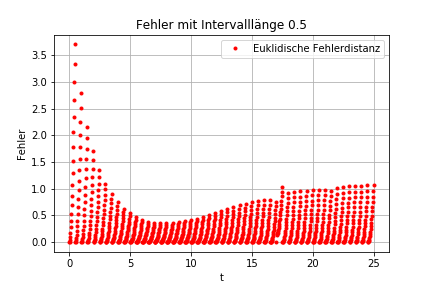
\includegraphics[scale=0.7]{papers/perturbation/bilder/halberintervall.png}
    \caption{Fehler bei halbierter Intervalldauer}
	\label{errorShortInterval}
\end{figure}

In einem zweiten Schritt haben wir die Intervallänge nochmals auf die Länge $\Delta t = 0.25$ halbiert. 
Dies ist in Abbildung \ref{errorShortInterval2} ersichtlich. 
Wir erhalten wieder einen Genaugikeitsgewinn um den Faktor 4 bzw. 2 Bit. 
Dies lässt sich leider jedoch nicht weiter beliebig fortsetzen. 
Die Rechenlast des Satelliten bleibt konstant und ist nicht von der Intervalllänge abhängig. 
Der Aufwand für die Bodenstation nimmt jedoch zu. 
Da die nummerischen Berechnungen für aufwänderige Formeln (wie Satellitenbahnen) oft ein wenig dauern und gegebenfalls viel Rechenpower benötigen, sind diese nicht günstig und können nicht beliebig oft ausgeführt werden.

\begin{figure}
    \centering
    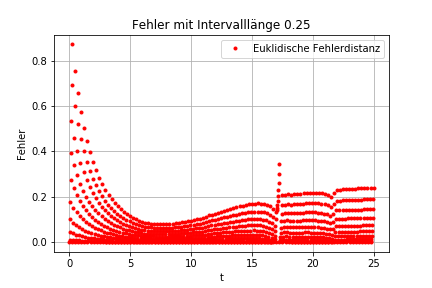
\includegraphics[scale=0.7]{papers/perturbation/bilder/viertelintervall.png}
    \caption{Fehler mit einem Viertel der Intervalldauer}
	\label{errorShortInterval2}
\end{figure}

\subsection{Erhöhung der Ordnung}
Eine andere Möglichkeit zur Steigerung der Genauigkeit eröffnet sich dadurch, dass man anstelle $x_0, y_0, v_{0_x}$ und $v_{0_y}$, was an sich Polynome nullter Ordnung sind, Polynome höherer Ordnung ansetzt. 
Wir schauen uns ein Beispiel erster Ordnung an. 
Um die Indizierung simpel zu halten, verwenden wir die Notation $x_0$ und $y_0$ wieder.
\[
\textcolor{red}{x_0 \longrightarrow x_0 +   x_1  \cdot \Delta t}
\]
\[
\textcolor{red}{y_0 \longrightarrow y_0 +   y_1  \cdot \Delta t}
\]
Die Anfangsbedingungen für die Geschwindigkeit, also $v_{0_x}$ und $v_{0_y}$, ergeben sich durch Ableiten des Ortes, also durch Ableiten obiger Gleichung nach $\Delta t$. 
Durch diesen Trick können wir die Anzahl der unbekannten Variablen im Rahmen halten.
\[
\textcolor{blue}{v_x \longrightarrow x_1}
\]
\[
\textcolor{blue}{v_y \longrightarrow y_1}
\]

Betrachten wir nun ein bestimmtes Intervall, etwa $t \in [5,6)$. Innerhalb dieses Intervalls arbeiten wir mit $t=5$, $\Delta t \in [0,1)$. 
$t$ wird also fixiert und $\Delta t$ ist unsere neue Variable. 
So gilt nach Einsetzen in Gleichungen \ref{eq:x_simple} und \ref{eq:y_simple} 
\begin{equation}\label{eq:x_ordnung1}
    x(t+ \Delta t) = \textcolor{red}{x_0 +   x_1  \cdot \Delta t} + \textcolor{blue}{x_1} \Delta t
\end{equation}
\begin{equation}\label{eq:y_ordnung1}
    y(t+ \Delta t) = \textcolor{red}{y_0 +   y_1  \cdot \Delta t} + \textcolor{blue}{y_1} \Delta t - \frac{1}{2}g \Delta t^2
\end{equation}

\subsubsection{Lösung des Problems mit linearer Interpolation}
In obiger Gleichung sind $x_0, x_1, y_0$ und $y_1$ Unbekannte, die es zu bestimmen gilt. 
Indem wir $\Delta t = 0$ setzen, erhalten wir auf relativ einfache Art und Weise $x_0$ und $y_0$.
\[
x_0 = x(t)
\]
\[
x_0 = y(t)
\]
Da die Bodenstation die exakte Position berechnen kann, können wir diese Werte direkt von der Bodenstation übernehmen. 
Nach kurzer Umformung ergibt sich für die zwei weiteren Unbekannten $x_1$ und $y_1$:
\[
x_1 = \frac{x(t + \Delta t) - x_0}{2 \Delta t}
\]
\[
y_1 = \frac{y(t + \Delta t) - y_0 + \frac{1}{2}g \Delta t ^2}{2 \Delta t}
\]
Wir können nun für $\Delta t$ einen beliebigen Wert wählen und so die verbleibenden Unbekannten bestimmen. 
Wählt man etwa $\Delta t = 1$, also die volle Intervalllänge, betreibt man lineare Interpolation und es ergibt sich der Fehler wie in Bild \ref{errorOrdnung1Linear} zu erkennen.

\begin{figure}
    \centering
    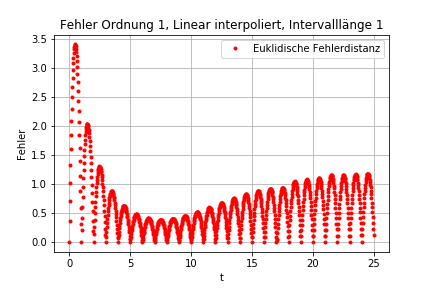
\includegraphics[scale = 0.7]{papers/perturbation/bilder/linear_error.png}
    \caption{Fehler bei linearer Interpolation}
	\label{errorOrdnung1Linear}
\end{figure}

Das zu beobachtende Fehlerverhalten macht durchaus Sinn. 
Da wir als Stützpunkte unserer Interpolation jeweils den Beginn und das Ende eines Intervalls der Dauer $t=1$ gewählt haben, ist der Fehler an den jeweiligen Stützstellen 0. 
Dazwischen nimmt er erst zu, erreicht sein Maximum in der Mitte des Intervalls, um anschliessend wieder abzunehmen.

Wir erkennen erneut, dass die Genauigkeit etwa 4x höher ist, als bei der Störungskorrektur nullter Ordnung. 
Das heisst, wir haben erneut 2 Bit Genauigkeit gewonnen. 
Selbstverständlich könnte man nun erneut die Intervalldauer reduzieren, um die Genauigkeit weiter zu erhöhen.

\subsubsection{Lösung des Problems mit Taylorreihen}
Anstelle von linearer Interpolation, kann man die Unbekannten $x_0, x_1, y_0$ und $y_1$ auch anders bestimmen. 
Wir können Gleichungen \ref{eq:x_ordnung1} und \ref{eq:y_ordnung1} als Taylorentwicklungen interpretieren. 
Leiten wir diese nach $\Delta t$ ab, erhalten wir das folgende System.

\begin{equation}\label{eq:x_taylor}
    \dot{x}(t+ \Delta t) = x_1 + x_1 = 2x_1
\end{equation}
\begin{equation}\label{eq:y_taylor}
    \dot{y}(t+ \Delta t) = y_1 + y_1 - g \cdot \Delta t = 2y_1 - g \cdot \Delta t
\end{equation}

Indem wir nun die Bodenstation um die Werte $x(t)$ und $x(t+0.0001)$ bitten, können wir die Ableitung nach x wie folgt annähern:
\[
    \dot{x}(t) \approx \frac{x(t+0.0001) - x(t)}{0.0001}
\]

Dieser Wert lässt sich nun in\ref{eq:x_taylor} einsetzen, und somit kann $x_1$ bestimmt werden. 
Die Rechnung für die y-Koordinate kann analog getätigt werden.

\begin{figure}
    \centering
    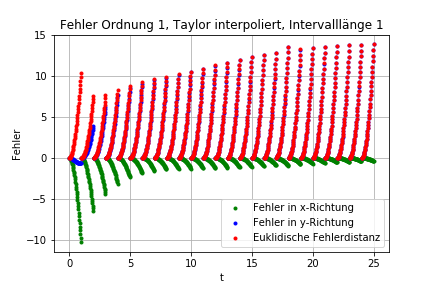
\includegraphics[scale = 0.7]{papers/perturbation/bilder/taylor_error.png}
    \caption{Fehler bei Interpolation mit Taylor}
	\label{errorOrdnung1Taylor}
\end{figure}

Beide Varianten, Interpolation und Taylorentwicklung, sind legitim. 
Die Interpolation ist am Anfang und Ende des Intervalles exakt, hat dafür aber in der Mitte einen relativ hohen Fehler. 
Die Taylorentwicklung ist vor allem zu Beginn des Intervalls exakt. 
Dies, da insbesondere bei höheren Ordnungen auch die Krümmung des Kurvenverlaufs berücksichtigt wird.
 Da sich allerdings alle Stützstellen am Anfang des Intervalles befinden, wird der Kurvenverlauf zum Ende des Intervalles hin immer ungenauer.